\documentclass[
%% TIKZ_CLASSOPTION %%
tikz
]{standalone}
\usepackage{amsmath}
\usetikzlibrary{matrix}
%% EXTRA_TIKZ_PREAMBLE_CODE %%
\begin{document}
%% TIKZ_CODE %%
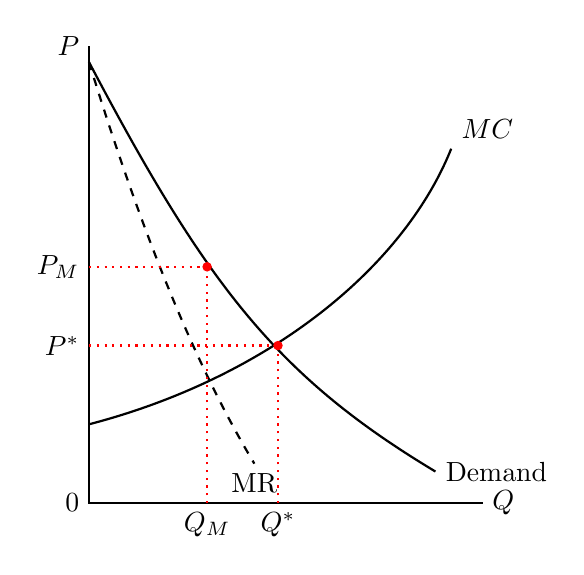
\begin{tikzpicture}[scale=1]
    % Axes
    \draw (0,5.8) node [left] {$P$} -- (0,0) node [left] {$0$} -- (5,0) node [right] {$Q$};
    
    % Labels for quantity
    \node [below] at (1.5,0) {$Q_M$};
    \node [below] at (2.4,0) {$Q^*$};

    % Labels for price
    \node [left] at (0,2) {$P^*$};
    \node [left] at (0,3) {$P_M$};

    % MC curve (Long-run supply)
    \draw[thick] (0,1) .. controls (2.3,1.6) and (4,3) .. (4.6,4.5) node [above right] {$MC$};

    % Demand curve
    \draw[thick] (0,5.6) .. controls (1.5,2.75) and (2.4,1.6) .. (4.4,0.4) node [right] {Demand};

    % MR curve
    \draw[thick, dashed] (0,5.6) .. controls (0.8,3) and (1.5,1.5) .. (2.1,0.5) node [below] {MR};

    % Vertical line at Q_M
    \draw[dotted, thick, red] (1.5,0) -- (1.5,3);

    % Vertical line at Q^*
    \draw[dotted, thick, red] (2.4,0) -- (2.4,2);

    % Horizontal lines for price
    \draw[dotted, thick, red] (0,3) -- (1.5,3);
    \draw[dotted, thick, red] (0,2) -- (2.4,2);

    % Points
    \filldraw[red] (1.5,3) circle (1.5pt); % Monopoly equilibrium
    \filldraw[red] (2.4,2) circle (1.5pt); % Competitive equilibrium
\end{tikzpicture}


\end{document}
